% Copyright 2008 by Till Tantau
%
% This file may be distributed and/or modified
%
% 1. under the LaTeX Project Public License and/or
% 2. under the GNU Free Documentation License.
%
% See the file doc/generic/pgf/licenses/LICENSE for more details.


\section{Introduction to Data Visualization}

\emph{Data visualization} is the process of converting \emph{data points,}
which typically consist of multiple numerical values, into a graphical
representation. Examples include the well-known function plots, but pie charts,
bar diagrams, box plots, or vector fields are also examples of data
visualizations.

The data visualization subsystem of \pgfname\ takes a general, open approach to
data visualization. Like everything else in \pgfname, there is a powerful, but
not-so-easy-to-use basic layer in the data visualization system and a less
flexible, but much simpler-to-use frontend layer. The present section gives an
overview of the basic ideas behind the data visualization system.


\subsection{Concept: Data Points}
\label{section-dv-intro-data-points}

The most important input for a data visualization is always raw data. This data
is typically present in different formats and the data visualization subsystem
provides methods for reading such formats and also for defining new input
formats. However, independently of the input format, we may ask what kind of
data the data visualization subsystem should be able to process. For
two-dimensional plots we need lists of pairs of real numbers. For a bar plot we
usually need a list of numbers, possibly together with some colors and labels.
For a surface plot we need a matrix of triples of real numbers. For a vector
field we need even more complex data.

The data visualization subsystem makes no assumption concerning which kind of
data is being processed. Instead, the whole ``rendering pipeline'' is centered
around a concept called the \emph{data point}. Conceptually, a data point is an
arbitrarily complex record that represents one piece of data that should be
visualized. Data points are \emph{not} just coordinates in the plane or the
numerical values that need to be visualized. Rather, they represent the basic
units of the data that needs to be visualized.

Consider the following example: In an experiment we drive a car along a road
and have different measurement instruments installed. We measure the position
of the car, the time, the speed, the direction the car is heading, the
acceleration, and perhaps some further values. A data point would consist of a
record consisting of a timestamp together with the current position of the car
(presumably two or three numbers), the speed vector (another two or three
numbers), the acceleration (another two or three numbers), and perhaps the
label text of the current experiment.

Data points should be ``information rich''. They might even contain more
information than what will actually be visualized. It is the job of the
rendering pipeline to pick out the information relevant to one particular data
visualization -- another visualization of the same data might pick different
aspects of the data points, thereby hopefully allowing new insights into the
data.

Technically, there is no special data structure for data points. Rather, when a
special macro called |\pgfdatapoint| is called, the ``totality'' of all
currently set keys with the |/data point/| prefix in the current scope forms
the data point. This is both a very general approach and quite fast since no
extra data structures need to be created.


\subsection{Concept: Visualization Pipeline}

The \emph{visualization pipeline} is a series of actions that are performed on
the to-be-visualized data. The data is presented to the visualization pipeline
in the form of a long stream of  complex data points. The visualization
pipeline makes several passes over this stream of data points. During the first
pass(es), called the \emph{survey phase(s)}, information is gathered about the
data points such as minimal and maximal values, which can be useful for
automatic fitting of the data into a given area. In the main pass over the
data, called the \emph{visualization phase}, the data points are actually
visualized, for instance in the form of lines or points.

Like as for data points, the visualized pipeline makes no assumptions
concerning what kind of visualization is desired. Indeed, one could even use it
to produce a plain-text table. This flexibility is achieved by extensive use of
objects and signals: When a data visualization starts, a number of signals (see
Section~\ref{section-signals} for an introduction to signals) are initialized.
Then, numerous ``visualization objects'' are created that listen to these
signals. These objects are all involved in processing the data points. For
instance, the job of an |interval mapper| object is to map one attribute of a
data point, such as a car's velocity, to another, such as the $y$-axis of a
plot. For each data point the different signals are raised in a certain order
and the different visualization objects now have a chance of preparing the data
point for the actual visualization. Continuing the above example, there might
be a second |interval mapper| that takes the computed $y$-position and applies
a logarithm to it, because a log-plot was requested. Then another mapper, this
time a |polar mapper| might be used to map everything to polar coordinates.
Following this, a |plot mark visualizer| might actually draw something at the
computed position.

The whole idea behind the rendering pipeline is that new kinds of data
visualizations can be implemented, ideally, just by adding one or two new
objects to the visualization pipeline. Furthermore, different kinds of plots
can be combined in novel ways in this manner, which is usually very hard to do.
For instance, the visualization pipeline makes it easy to create, say,
polar-semilog-box-plots. At first sight, such new kinds of plots may seem
frivolous, but data visualization is all about gaining insights into the data
from as many different angles as possible.

Naturally, creating new classes and objects for the rendering pipeline is not
trivial, so most users will just use the existing classes, which should, thus,
be as flexible as possible. But even when one only intends to use existing
classes, it is still tricky to setup the pipeline correctly since the ordering
is obviously important and since things like axes and ticks need to be
configured and taken care of. For this reason, the frontend libraries provide
preconfigured rendering pipelines so that one can simply say that a data
visualization should look like a |line plot| with |school book axes| or with
|scientific axes|, which selects a certain visualization pipeline that is
appropriate for this kind of plot:
%
\begin{codeexample}[setup code]
    \usetikzlibrary{datavisualization.formats.functions}
\end{codeexample}
%
\begin{codeexample}[]
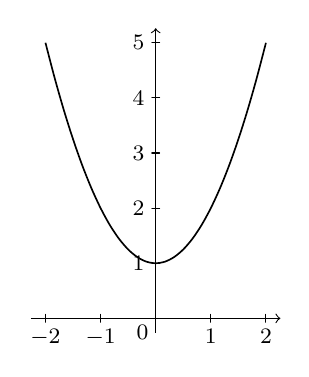
\begin{tikzpicture}[scale=.7]
  \datavisualization [school book axes, visualize as smooth line]
  data [format=function] {
    var x : interval [-2:2];
    func y = \value x*\value x + 1;
  };
\end{tikzpicture}
\end{codeexample}
%
\begin{codeexample}[]
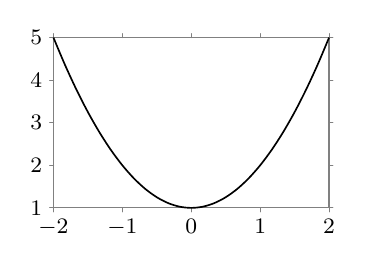
\begin{tikzpicture}[scale=.7]
  \datavisualization [scientific axes, visualize as smooth line]
  data [format=function] {
    var x : interval [-2:2];
    func y = \value x*\value x + 1;
  };
\end{tikzpicture}
\end{codeexample}
%
One must still configure such a plot (choose styles and themes and also specify
which attributes of a data point should be used), but on the whole the plot is
quite simple to specify.


%%% Local Variables:
%%% mode: latex
%%% TeX-master: "pgfmanual"
%%% End:
